\documentclass[]{article}
\usepackage[a4paper]{geometry}
\usepackage{amssymb}
\usepackage{amsmath}
\usepackage{mathabx}
\usepackage{graphics}
\usepackage{mathtools}
\usepackage{tikz}
\usepackage{array}
\usepackage{proof}
\usepackage{hyperref}
\definecolor{linkcolour}{rgb}{0,0.2,0.6}
\hypersetup{colorlinks,breaklinks,urlcolor=linkcolour,linkcolor=linkcolour}

\begin{document}
\author{Merle Beaujon [6050417], Konstantinos Kogkalidis [6230067]}
\title{Commonsense Reasoning and Argumentation}
\maketitle
\section{Introduction}
\subsection{Preface}
In this exercise, we model a conflict-of-opinion argument between two parties using the ASPIC+ framework. Motivated by recent events and discussions, we choose to have the argument revolve around gun laws in the U.S.A.; in particular, one party proposes stricter gun control rules, whereas the other party opposes gun control\footnote{The opinions voiced by the parties do not represent either of the students' beliefs.}. Obviously, the scope of this exercise is limited; we do not hope to encapsulate within our example the full depth of the issue (neither attempt to do so), but rather show how ASPIC\texttt{+}\cite{ASPIC} could potentially be used to model relative argument strength in complex sociopolitical matters.
\subsection{Contents}
Section \ref{sec2} presents a natural language version of the argument. In Section \ref{sec3} we briefly discuss the ASPIC\texttt{+} modeling of our argument and some design choices we made. 

\section{Natural Language Argument}\label{sec2}
We denote the proponent by \textbf{P} and the oponent by \textbf{O}. This version does not follow a protocol or scheme in particular, instead prioritizing naturality and coherence.

\begin{itemize}
\item[\textbf{P}]  \textit{Gun regulations should be more strict.}
\item[\textbf{O}]  \textit{Gun regulations should not be more strict, because it is a fundamental right to own a gun as stated in the United States Bill of Rights.}
\item[\textbf{P}]  \textit{The Bill of Rights was written more than two centuries ago, when guns were far less dangerous. It is outdated and therefore unapplicable in this case.}
\item[\textbf{O}]  \textit{It's fairly outdated, that is true; however the Supreme Court has reaffirmed this right in 2002.}
\item[\textbf{P}] \textit{ Well ok, but would you agree that the USA is a democracy and in a democracy the laws should serve the public interest?}
\item[\textbf{O}]  \textit{Okay..}
\item[\textbf{P}]  \textit{Well, 48\% of the population wishes for the gun rules to be stricted, against 30\% that has no opinion and 22\% that wants them less strict. So the population wishes for gun rules to be stricter.}
\item[\textbf{O}]  \textit{That might be the case, and I concede that the larger group does wish for stricter rules. However, 48\% is not a majority, so you can't conclude that the the population in general wishes for stricter gun laws.}
\item[\textbf{P}]  \textit{Still, current laws make private gun ownership easy, leading to many guns, which in turn result to more deaths. So we should strengthen gun regulations. }
\item[\textbf{O}]  \textit{Why do you think more guns lead to more deaths?}
\item[\textbf{P}]  \textit{Well, police reports that 60\% of the homicides are perpetrated with a handgun. You must see the correlation there, right?}
\item[\textbf{O}]  \textit{Yes, but recent research states that there is not enough evidence to conclude a causative relation between the two.}
\item[\textbf{P}] \textit{Fair point. How about suicides though? Again, police reports a high percentage of suicices being commited with a gun.}
\item[\textbf{O}]  \textit{But South Korea has far more suicides per population sample even though guns are banned there; so I don't see a causation here either.}
\item[\textbf{P}]  \textit{So what about gun related lethal accidents? Newspapers often report those.}
\item[\textbf{O}]  \textit{That's true I guess. On the other hand, gun posession can deter violent crime, increasing public safety.}
\item[\textbf{P}] \textit{ I think it's the other way around; gun posession enables violent crime, decreasing public safety.}
\item[\textbf{O}]  \textit{We agree to disagree, I suppose.}
\end{itemize} 

\section{ASPIC\texttt{+} Model}\label{sec3}
\subsection{TOAST Implementation}
An implementation of our model on TOAST\cite{TOAST} can be found at \url{http://toast.arg-tech.org/14578}.
\subsection{Design Choices}
Our original idea was to instantiate our model with no defeasible rules, instead using material implication in the ordinary premises $\mathcal{K}_p$ to model non-monotonic reasoning. Similarly, we planned to have the strict rules be all well-formed formulae of first-order logic, and move domain-specific object properties and relations to the axiom belief set $\mathcal{K}_n$. The reasoning for this would be to allow for contraposition and undercutting to be modeled clasically. However this approach was quickly abandoned due to limitations of TOAST as well as issues mentioned in chapter 6.4 of the course reader. Specifically, TOAST is unable to handle first-order formulae including quantification, forcing us to explicitly define properties and relations on a per-object basis.

To facilitate argument building, some of the defeasible rules are instead written as ordinary premises, for instance \textit{GunsToSuicides} $\in \mathcal{K}_p$ could also be read as $Guns \supset Suicides \in \mathcal{K}_p$. 

The elements of our axiom belief base are either facts that cannot be argued about (at least in our simplified model of the world), i.e. the fact that the USA is a democracy or that murder is a deadly event- but also knowledge that we want to treat as shared by both parties and mutually accepted, such as the common knowledge of police and scientific reports. 
\subsection{Preferences, Link Orderings and Results}
We constructed preferences between rules that both abide by our intuitions and are as unbiased as possible. By that notion, we have set the following preferences:
\begin{enumerate}
\item \textsc{r3} $<$ \textsc{r2} (Non-majority vs. Largest group)\\
The \textit{not-majority} argument inhibits argumentation and is not grounded; a group majority does not have to be a percentile majority to affect policy making.
\item \textsc{r8} $<$ \textsc{r13} (Police reports vs. Academic papers)\\
The correlation stated by the police does not equal causation; even though one is an indicator of the other, the lack of evidence cited by scientific reports effectively stops the ability to argue further about gun ownership increasing homicides.
\item \textsc{r18} $<$ \textsc{r19} (Preventing crime vs. Enabling crime)\\
We simply think that even though both arguments are solid, guns preventing crime but also enabling it nullifies the former argument, allowing for a rule preference to be applicable in the latter's favor.
\end{enumerate}

We chose last link ordering as our ordering method; this only affects a single argument, namely the \textit{no guns yet suicides in korea} against \textit{guns lead to suicides}. Our choice for last link ordering is justified by the fact that the former argument is essentially anecdotal evidence against a defeasible generalization that already exists in the premises- therefore it would make no sense for them to be on equal grounds. It is important to note here that TOAST does not apply link ordering according to the reader's definition; weakest link ordering for firm arguments, and last link for argument pairs where one argument has no defeasible rules are not properly treated. 

Our argumentation scheme, despite its naivety and simplified nature, displays an interesting property; the major blocker toward gun regulations is the constitution and its' treatment of gun ownership as an irrevokable individual right. Arguing about the constitution's applicability is much more difficult than arguing about the effects of gun ownership. Additionally, regardless of how strong the rest of the argumentation of the proponent is, the constitution move guarantees non-justifiability of the proponent's argument in grounded semantics while requiring minimal effort from the oponent. This difficulty is not just local to our presented argument but also coincides with the real world as evidenced by recent political discussions on the topic.

\subsection{Argument Graph}
The below figures depict the argument structures of all possible arguments for and against stricter gun laws, and their attack relations. For readability, inter-argument attacks are denoted by arrows from and towards argument names. Unsuccessful attack relations are displayed by a dotted arrow undercut by two slashes.

\begin{figure}
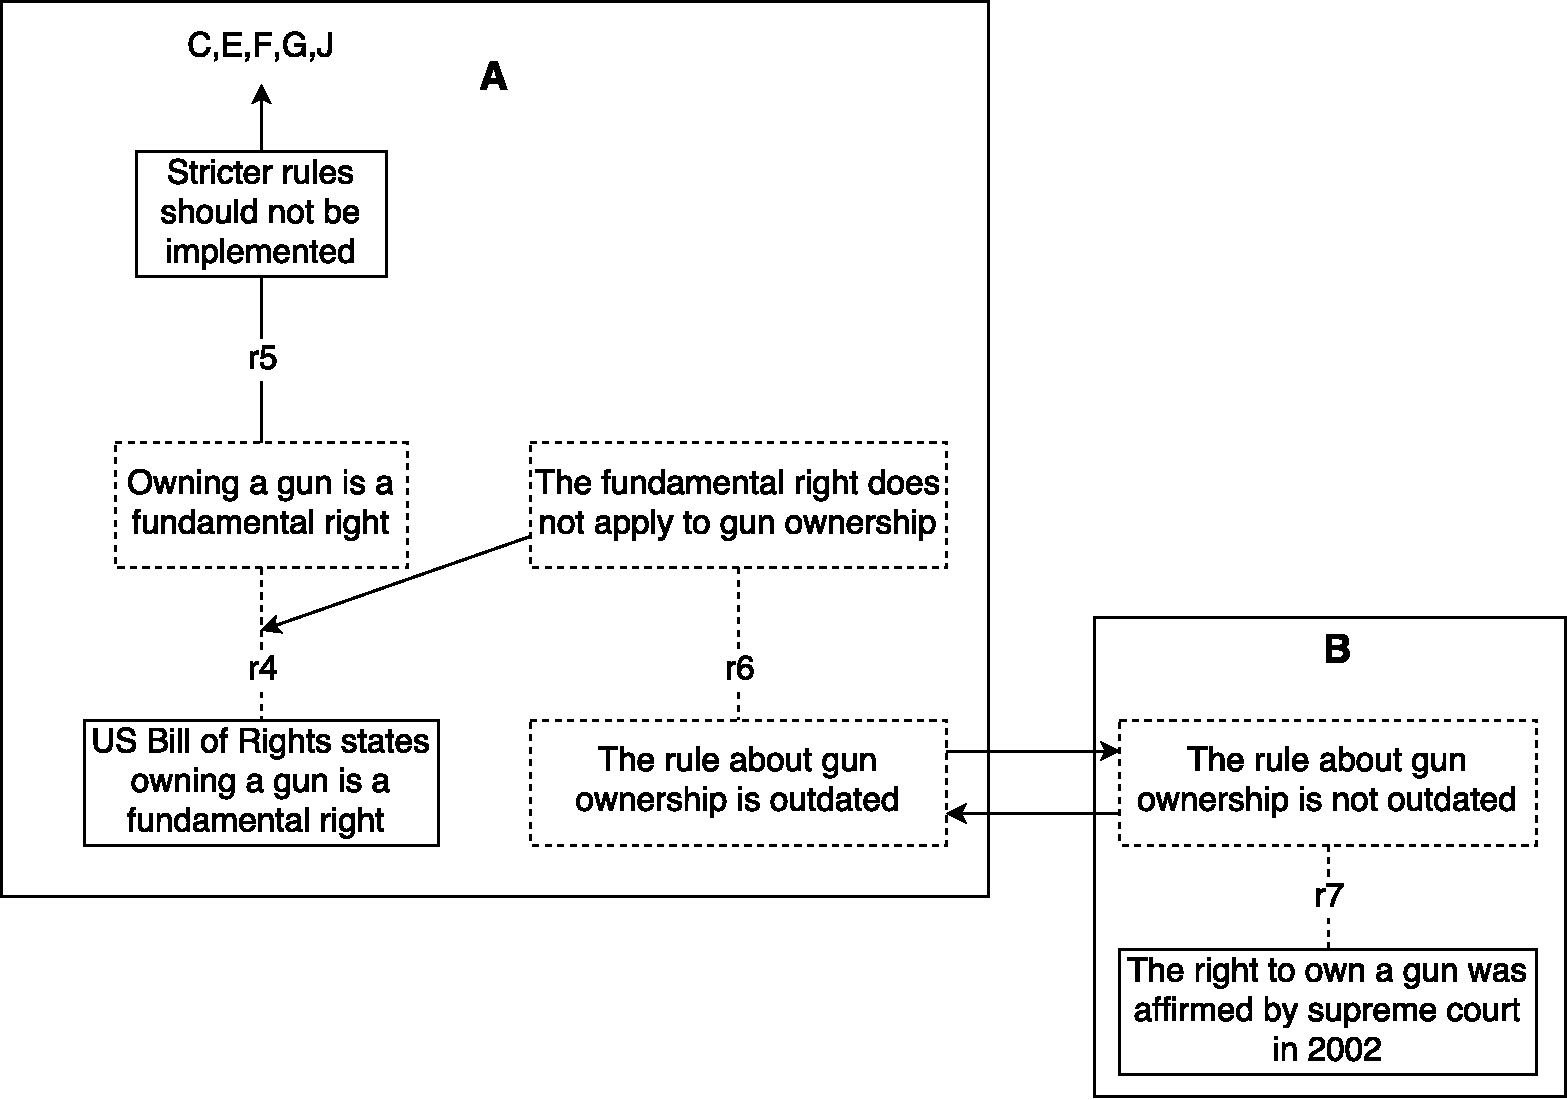
\includegraphics[scale=0.5]{images/AB.pdf}
\caption{Arguments A and B (on the applicability of the constitutional law).}
\end{figure}
\begin{figure}
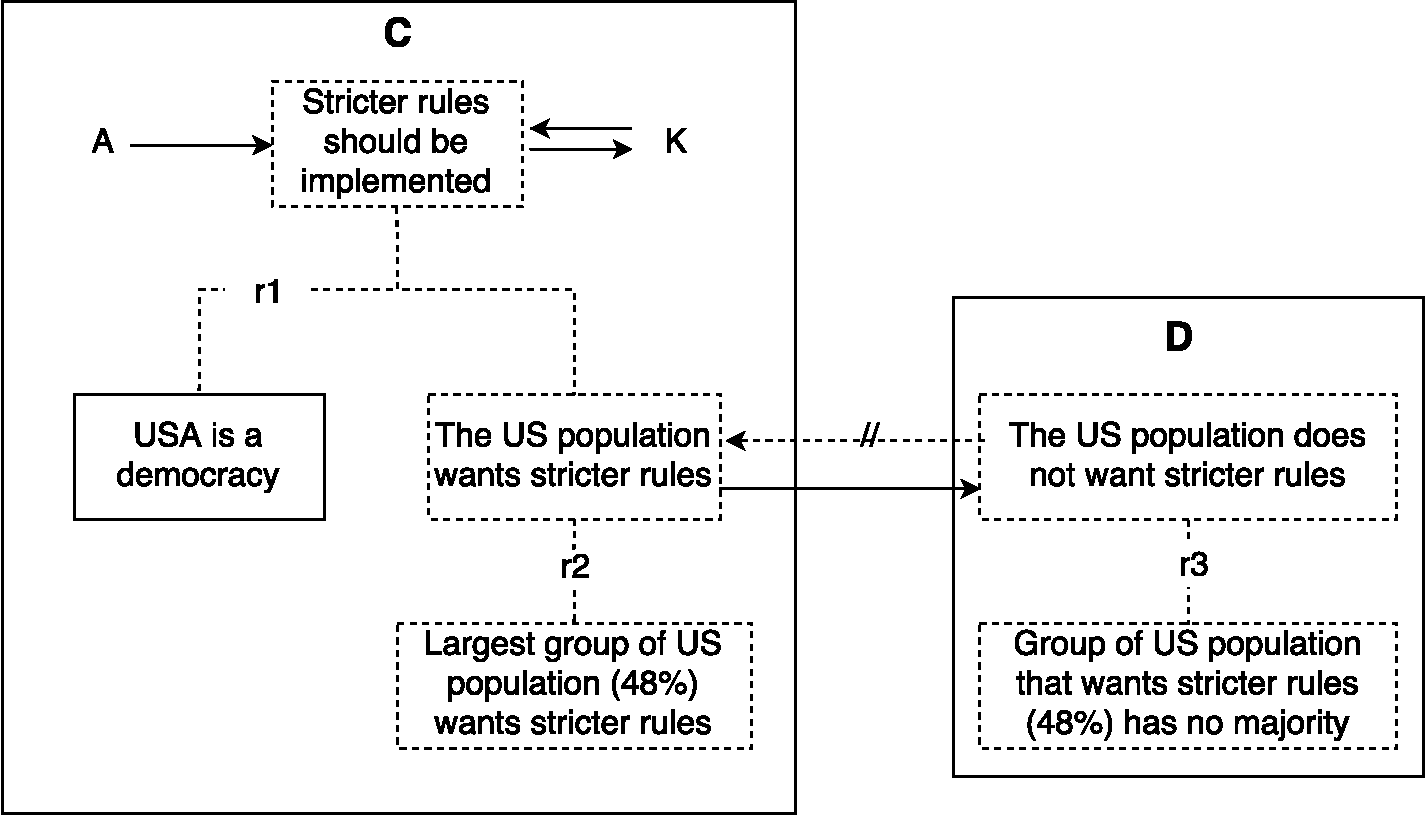
\includegraphics[scale=0.5]{images/CD.pdf}
\caption{Arguments C and D (on popular opinion)}
\end{figure}
\begin{figure}
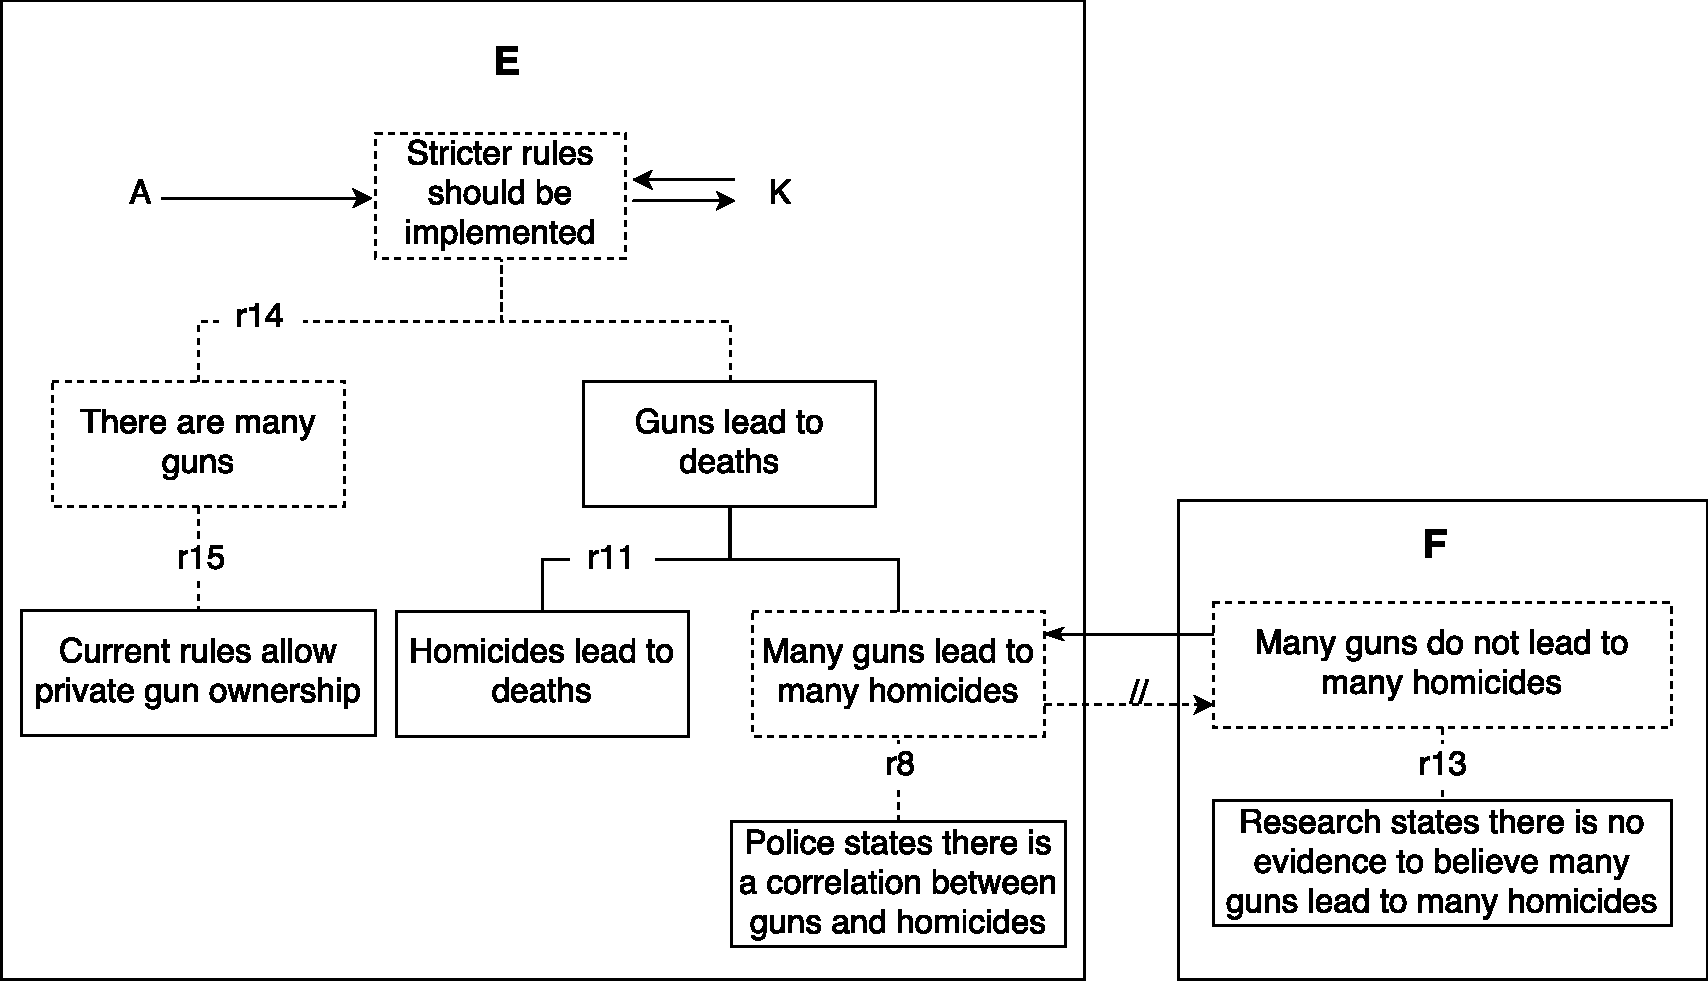
\includegraphics[scale=0.5]{images/EF.pdf}
\caption{Arguments E and F (on homicides)}
\end{figure}
\begin{figure}
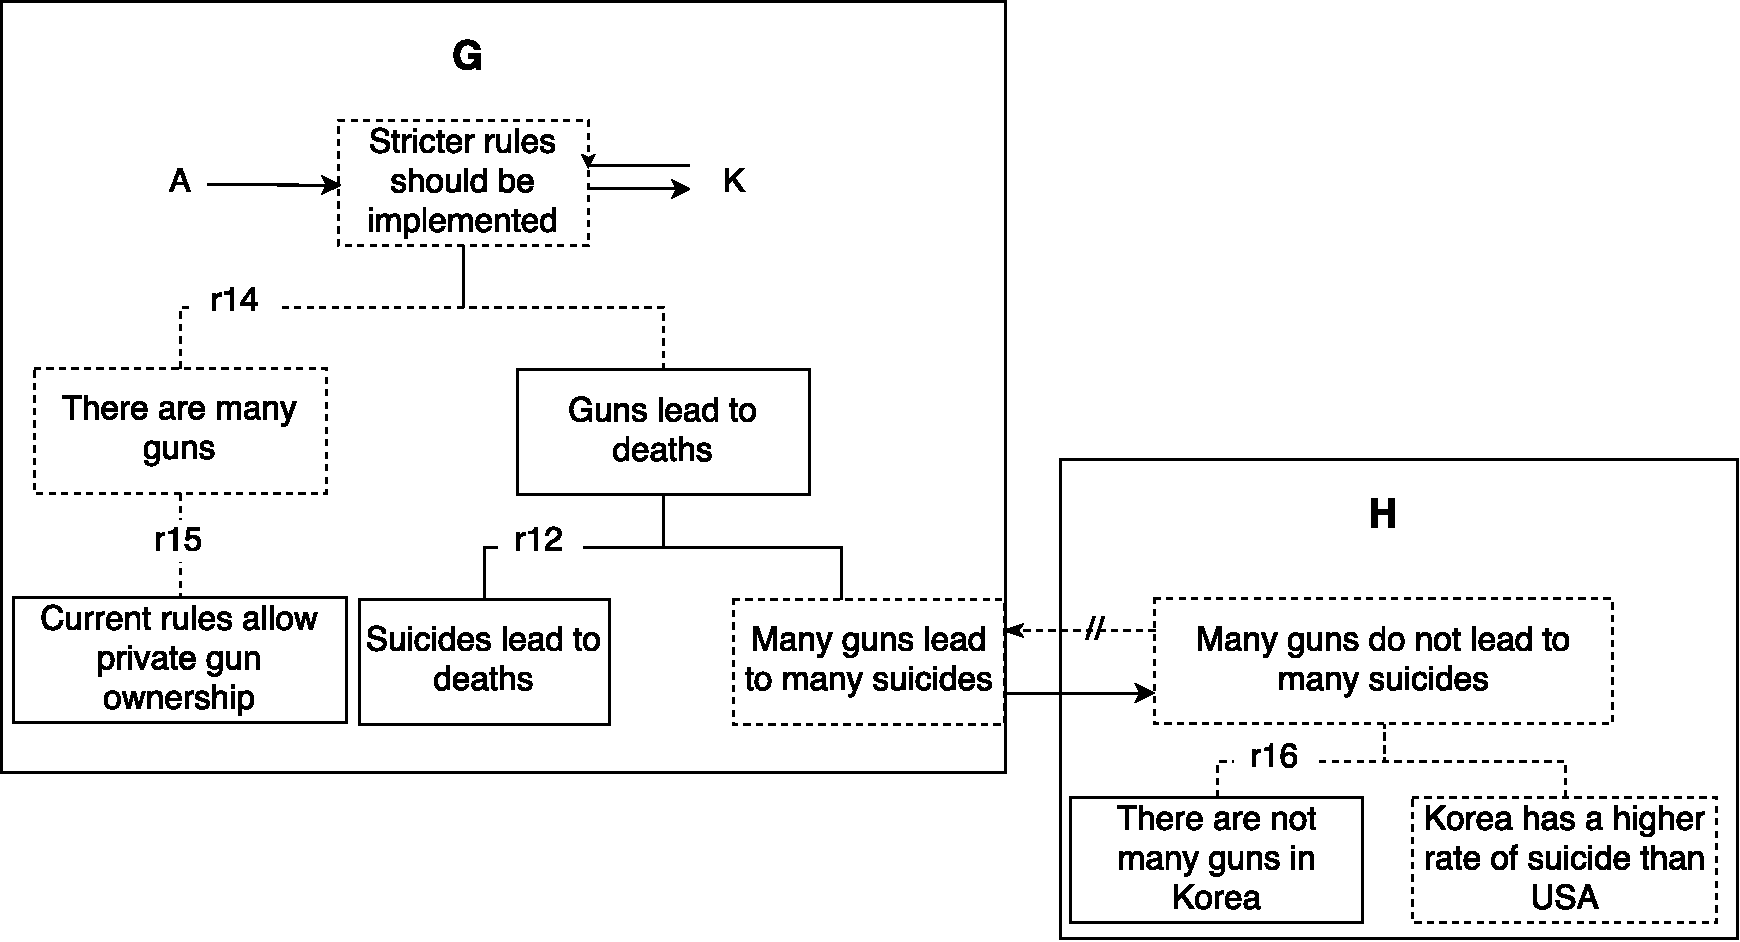
\includegraphics[scale=0.5]{images/GH.pdf}
\caption{Arguments G and H (on suicides)}
\end{figure}
\begin{figure}
\begin{center}
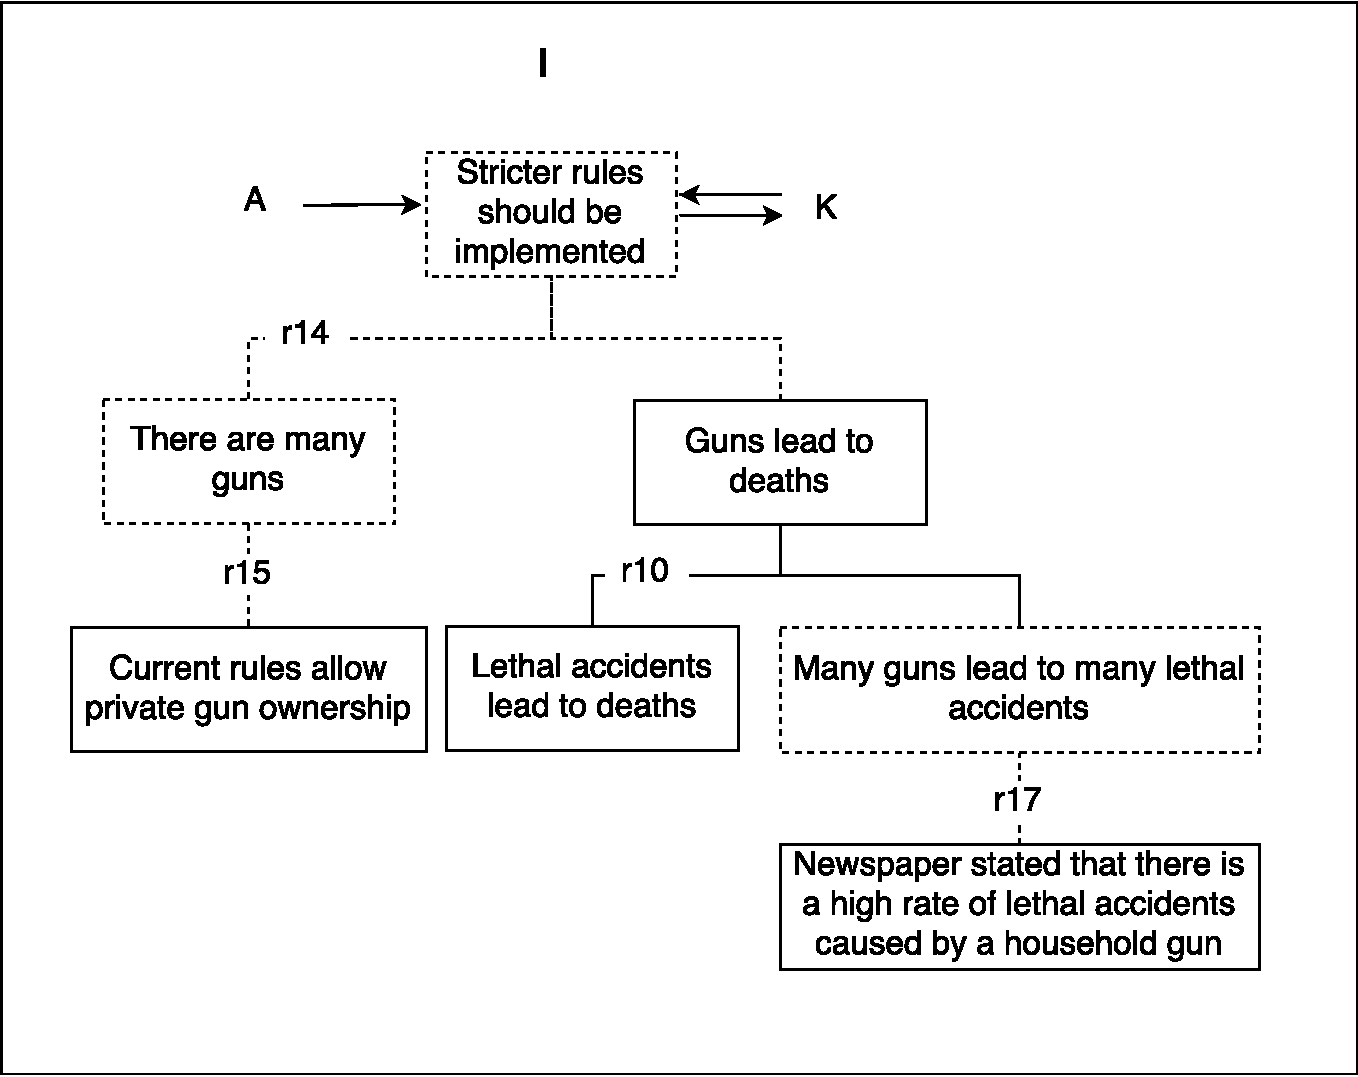
\includegraphics[scale=0.5]{images/I.pdf}
\end{center}
\caption{Argument I (on lethal accidents)}
\end{figure}
\begin{figure}
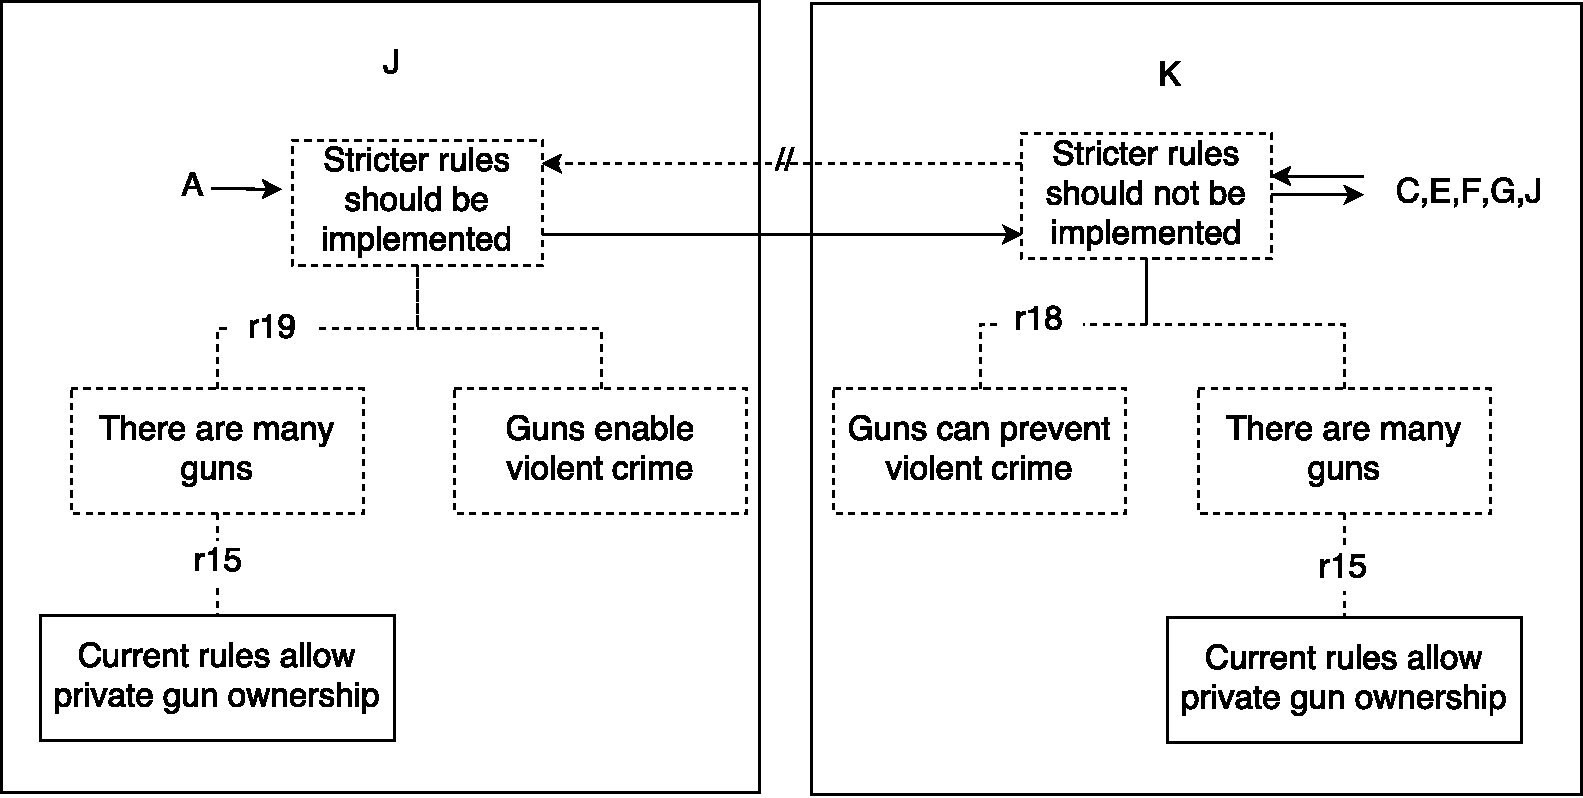
\includegraphics[scale=0.5]{images/JK.pdf}
\caption{Arguments J and K (on violent crime)}
\end{figure}

\bibliographystyle{ieeetr}
\bibliography{sources}
\end{document}
